\section{Tension Resolution}
The advantage of tension avoidance is that it is simple. The disadvantage is
that it requires large fast Phase 2 quorums. In this section, we explain how to
implement a multi-leader generalized state machine replication protocol using
\defword{tension resolution}. Tension resolution is significantly more
complicated than tension avoidance, but it does not require large fast Phase 2
quorums.

Instead of avoiding the tension between the consensus and dependency invariant,
tension resolution uses additional machinery to resolve it when it arrives.
Consider a scenario where a proposer $p$ is forced to propose a set of
$\deps{v_x}$ in round $i$ to maintain the consensus invariant because
$\deps{v_x}$ may have been chosen in a previous round. Simultaneously, $p$ is
forced not to propose $\deps{v_x}$ because it cannot guarantee that
$\deps{v_x}$ was computed by a majority of the dependency service nodes. This
is the moment of tension that tension avoidance avoids. Tension resolution, on
the other hand, allows this to happen. When it does, the proposer $p$ leverages
additional machinery built into the protocol to determine either that (a)
$\deps{v_x}$ was not chosen or (b) $\deps{v_x}$ was computed by a majority of
dependency service nodes.

We introduce Majority Commit \BPaxos{}, a protocol that implements tension
resolution. We then discuss the protocol's relationship with
EPaxos~\cite{moraru2013there} and Caesar~\cite{enes2020state}.

\subsection{Pruned Dependencies}
Before we discuss Majority Commit \BPaxos{}, we introduce the notion of pruned
dependencies. Imagine a proposer $p$ sends command $x$ to the dependency
service in vertex $v_x$, and the dependency service computes the dependencies
$\deps{v_x}$. Let $v_y \in \deps{v_x}$ be one of $v_x$'s dependencies. To
maintain the dependency invariant, all of the protocols that we have discussed
thus far would get $v_x$ chosen with a dependency on $v_y$, but this is not
always necessary.

Assume that that the proposer $p$ knows that $v_y$ has been chosen with command
$y$ and dependencies $\deps{v_y}$. Further assume that $v_x \in \deps{v_y}$.
That is, $v_y$ has already been chosen with a dependency on $v_x$. In this
case, there is no need for $v_x$ to depend on $v_y$. The dependency invariant
asserts that if two vertices $v_a$ and $v_b$ are chosen with conflicting
commands $a$ and $b$, then either $v_a \in \deps{v_b}$ or $v_b \in \deps{v_a}$.
Thus, in our example, if $v_y$ has already been chosen with a dependency on
$v_x$, then there is no need to propose $v_x$ with a dependency on $v_y$.

Similarly, if $v_y$ has been chosen with $\noop$ as part of a recovery, then
there is no need to propose $v_x$ with a dependency on $v_y$ because $x$ and
$\noop$ do not conflict.

Let $\deps{v_x}$ be a set of dependencies computed by the dependency service.
Let $P \subseteq \deps{v_x}$ be a set of vertices $v_y$ such that $v_y$ has
been chosen with $\noop$ or $v_y$ has been chosen with $v_x \in \deps{v_y}$. We
call $\deps{v_x} - P$ the \defword{pruned dependencies} of $v_x$ with respect
to $P$. Majority Commit \BPaxos{} maintains \invref{PrunedDependencies}, the
\defword{pruned dependency invariant}. The pruned dependency invariant is a
relaxation of the dependency invariant. If a protocol maintains the pruned
dependency invariant, it is guaranteed to maintain the dependency invariant.

\begin{invariant}[Pruned Dependency Invariant]\invlabel{PrunedDependencies}
  For every vertex $v_x$, either $(\noop, \emptyset{})$ is chosen in $v_x$ or
  $(x, \deps{v_x} - P)$ is chosen in $v_x$ where $\deps{v_x}$ are dependencies
  computed by the dependency service and where $\deps{v_x} - P$ are the pruned
  dependencies of $v_x$ with respect to some set $P$.
\end{invariant}

\subsection{Majority Commit \BPaxos{}}
For clarity of exposition, we first introduce a version of Majority Commit
\BPaxos{} that can sometimes deadlock. Later, we modify the protocol to
eliminate the possibility of deadlock.

Majority Commit \BPaxos{} is identical to Fast \BPaxos{} except for the
following two modifications.
%
First, every Fast Paxos acceptor maintains a conflict graph in exactly the same
way as the replicas do. That is, when an acceptor learns that a vertex $v_x$
has been chosen with command $x$ and dependencies $\deps{v_x})$, it adds $v_x$
to its conflict graph with command $x$ and with edges to every vertex in
$\deps{v_x}$. We will see momentarily that whenever a Majority Commit \BPaxos{}
proposer sends a \msgfont{Phase2a} message to the acceptors with value $v = (x,
\deps{v_x} - P)$, the proposer also sends $P$ and all of the commands and
dependencies chosen in in the vertices in $P$. Thus, when an acceptor receives
a \msgfont{Phase2a} message, it updates its conflict graph with the values
chosen in $P$.
%
Second and more substantially, a proposer executes a significantly more complex
recovery procedure. This is shown in \algoref{MajorityCommitBPaxos}.

\section{Deadlock Bipartisan Paxos}
In this section, we present \defword{Deadlock Bipartisan Paxos}. Deadlock
BPaxos can commit commands in one round trip like Unanimous BPaxos, but
Deadlock BPaxos only requires a superquorum size of $f + \floor{\frac{f}{2}} +
1$. Unfortunately, there are situations in which Deadlock Paxos can deadlock.
We will fix this pesky liveness problem in the next section.

\paragraph{Ordering Service}
Deadlock BPaxos uses the same ordering service as BPaxos and Unanimous BPaxos.

\paragraph{Consensus Service}
Deadlock BPaxos uses the same consensus service as Unanimous BPaxos, except
that Deadlock BPaxos uses a superquorums size of $f + \floor{\frac{f}{2}} + 1$,
the same as regular Fast Paxos.

\paragraph{Overview}
In the normal case, Deadlock BPaxos nodes behave exactly like Unanimous BPaxos
nodes. Upon receiving a command $a$ from a client, a Deadlock BPaxos node $R$
chooses some previously unused instance $R.i$ for the command. It then sends
$(R.i, a)$ to the ordering service nodes.
%
When an ordering service node $o_j$ receives $(R.i, a)$, it proposes it's reply
$(R.i, a, \deps{a}_j)$ to $p_j$, the colocated Paxos acceptor. $p_j$ then sends
its vote back to $R$.
%
If $R$ receives a superquorum of matching votes $(R.i, a, \deps{a})$, then the
gadget is considered chosen. If it does not receive a superquorum of matching
votes, it enters recovery.

Recovery is where Deadlock BPaxos differs from the incorrect BPaxos variant in
\secref{IncorrectBPaxos} and from Unanimous BPaxos. Deadlock BPaxos proposers
implement Case 2 and Case 3 of \algoref{FastPaxosTweak} as described in
\algoref{DeadlockBPaxos}. The bulk of the complexity comes from resolving the
tension between maintaining \invref{GadgetsChosen} and
\invref{ConflictingGadgets}, as exemplified by the upper right corner of
\figref{BPaxosLogic}.

\paragraph{Pruned Dependencies}
We'll walk through \algoref{DeadlockBPaxos} momentarily, but first we pause to
understand one of the key invariants that it maintains. Recall that in order to
preserve \invref{ConflictingGadgets}, both BPaxos and Unanimous BPaxos maintain
the invariant that a proposer can only propose a value $(a, \deps{a})$ if
either $\deps{a}$ is a response from the ordering service or if $(a, \deps{a})
= (\noop, \emptyset)$.

Deadlock BPaxos does not maintain this invariant, Instead, it maintains an
invariant that is slightly weaker but still strong enough to imply
\invref{ConflictingGadgets}. The motivation for the weaker invariant is as
follows. Imagine a Deadlock BPaxos node $R$ sends command $a$ to the ordering
service in instance $I_a$, and the ordering service responds with $(I_a, a,
\deps{a})$. Let $I_b \in \deps{a}$ be one of $a$'s dependencies. Assume that
that $R$ knows that $I_b$ has been committed with command $b$ and dependencies
$\deps{b}$. Further assume that $I_a \in \deps{b}$. That is, there is an edge
from $I_b$ to $I_a$. In this case, there is no need for $R$ to include $I_b$ in
the dependencies of $I_a$! \invref{ConflictingGadgets} asserts that if two
committed commands conflict, one has an edge to the other (or both). If $I_b$
has already committed with an edge to $I_a$, there is no need to propose an
edge from $I_a$ back to $I_b$.
%
Similarly, if $I_b$ has been committed with a $\noop$, then there is no need to
propose an edge from $I_a$ to $I_b$ at all because $a$ and $\noop$ do not
conflict.

Let $(I_a, a, \deps{a})$ be a response from the ordering service. Let
$\Pnoop{a}$ be a set of instances $I_c$ in $\deps{a}$ such that $I_c$ has been
committed as a $\noop$. Similarly, let $\Pnotnoop{a}$ be a set of instances
$I_c$ in $\deps{a}$ such that $I_c$ has been committed with $I_a$ in
$\deps{c}$. Note that in this case, $c$ is not a $\noop$. We call
$\pruned(\deps{a}) = \deps{a} - (\Pnoop{a} \cup \Pnotnoop{a})$ the
\defword{pruned dependencies} of $I_a$ (or sometimes the pruned dependencies of
$a$ if $I_a$ is clear from context).  Deadlock BPaxos maintains the following
invariant:

\begin{boxedinvariant}\invlabel{PrunedDependencies}
  In Paxos instance $I_a$, A Deadlock BPaxos node will only propose a value of
  the form $(a, \pruned(\deps{a}))$ where $\pruned(\deps{a})$ is a pruned
  response from the ordering service or a value of the form $(\noop,
  \emptyset)$.
\end{boxedinvariant}

\invref{GadgetsChosen} and \invref{PrunedDependencies} imply
\invref{ConflictingGadgets}. To see why, consider two conflicting commands $a$
and $b$ chosen in instances $I_a$ and $I_b$ with pruned dependencies
$\pruned(\deps{a})$ and $\pruned(\deps{b})$ derived from unpruned dependencies
$\deps{a}$ and $\deps{b}$ from the ordering service. We want to show that $I_a
\in \pruned(\deps{a})$ or $I_b \in \pruned(\deps{a})$, or both. Note that $a$
and $b$ conflict, so we know that neither is a $\noop$ and that their unpruned
dependencies are from the ordering service.
%
By \invref{OrderingService}, either $I_b \in \deps{a}$ or $I_a \in \deps{b}$ or
both. Without loss of generality, assume $I_b \in \deps{a}$. If $I_b$ is also
in $\pruned(\deps{a})$, then we're done. Otherwise, $I_b$ has been pruned from
$\deps{a}$. This happens only if $b$ is a $\noop$ or if $I_b$ has been chosen
with $I_a \in \deps{b}$. $b$ is not a $\noop$, so $I_a \in \deps{b}$, and we're
done.

We'll see momentarily in \algoref{DeadlockBPaxos} that it's sometimes necessary
for a BPaxos node to know the sets $\Pnoop{-}$ and $\Pnotnoop{-}$ that have
been pruned from an ordering service response. Thus, BPaxos nodes propose
values of the form $(a, \pruned(\deps{a}), \Pnoop{a}, \Pnotnoop{a})$ to the
consensus service (instead of just $(a, \pruned(\deps{a}))$) where $\Pnoop{a}$
and $\Pnotnoop{a}$ were the instances pruned from $\deps{a}$ to get
$\pruned(\deps{a})$. That is, $\pruned(\deps{a}) = \deps{a} - (\Pnoop{a} \cup
\Pnotnoop{a})$. Note that when an ordering service node $o_j$ proposes value
$(a, \deps{a})$ to its colocated Fast Paxos acceptor, it actually proposes
value $(a, \deps{a}, \emptyset, \emptyset)$.

\paragraph{Deadlock BPaxos Nodes}
\begin{algorithm}[ht]
  \caption{Deadlock BPaxos recovery for instance $R.i$ (Case 2 and Case 3)}%
  \algolabel{DeadlockBPaxos}
  \begin{algorithmic}[1]
    \If{%
      $\nexists v \in V$ such that at least $\QuorumMajoritySize$ acceptors in
      $\quorum$ voted for $v$
    }
      \State propose anything that satisfies \invref{PrunedDependencies}
    \EndIf{}

    \State
    \State $(a, \deps{a}, \emptyset, \emptyset) \gets$ the value
             voted by at least $\QuorumMajoritySize$ acceptors in $\quorum$
    \State Send $(R.i, a)$ to the quorum $\quorum$ of ordering service nodes
    \State $\deps{a}' \gets$ the union of ordering service responses

    \State
    \If{$\deps{a} = \deps{a}'$}
      \State propose $(a, \deps{a}, \emptyset, \emptyset)$
    \EndIf{}

    \State
    \State $\Pnoop{a} \gets \emptyset$
    \State $\Pnotnoop{a} \gets \emptyset$
    \For{$I_b \in \deps{a}' - \deps{a}$}
      \If{$I_b$ not committed}
        \State recover $I_b$
      \EndIf
      \If{$I_b$ committed with $\noop$}
      \State $\Pnoop{a} \gets \Pnoop{a} \cup \set{I_b}$
        \State continue
      \EndIf{}
      \If{$I_b$ committed with $R.i \in \pruned(\deps{b})$}
        \Comment{$b \to a$ unpruned}
        \State $\Pnotnoop{a} \gets \Pnotnoop{a} \cup \set{I_b}$
        \State continue
      \ElsIf{$I_b$ committed with $R.i \notin \Pnotnoop{b}$}
        \Comment{$b \not\to a$}
        \State propose anything that satisfies \invref{PrunedDependencies}
      \Else{}
        \Comment{$b \not\to a$ pruned}
        \State $I_b$ committed with $R.i \in \Pnotnoop{b}$
        \State abort recovery; $R.i$ has already been chosen
      \EndIf{}
    \EndFor{}
    \State propose $(a, \deps{a}, \Pnoop{a}, \Pnotnoop{a})$
  \end{algorithmic}
\end{algorithm}

Now, we walk through \algoref{DeadlockBPaxos} for a Deadlock BPaxos node $S$
recovering instance $R.i$. If there does not exist a value $v \in V$ with at
least $\QuorumMajoritySize$ votes from acceptors in $\quorum$, then no value
could have been chosen in round $0$, so $S$ is free to propose anything, so
long as it satisfies \invref{PrunedDependencies}.

Otherwise, there is some $(a, \deps{a}, \emptyset, \emptyset)$ that was voted
by a majority of $\quorum$. We know that $\deps{a}$ is unpruned and that
$\Pnoop{a} = \Pnotnoop{a} = \emptyset$ because this value was proposed by an
ordering service node in round $0$.
%
As we saw with the incorrect BPaxos variant in \secref{IncorrectBPaxos}, we
cannot blindly propose $(a, \deps{a})$ because it's possible that $\deps{a}$ is
not a response from the ordering service.  Thus, $S$ has to do a bit of
detective work to determine either that $\deps{a}$ is indeed a response from
the ordering service or that $(a, \deps{a}, \emptyset, \emptyset)$ was
definitely not chosen.

First, $S$ sends $(R.i, a)$ to every ordering service node in $\quorum$ and
gathers the union of their responses, $\deps{a}'$. Note that these requests can
be piggybacked on the phase 1a messages previously sent by $S$ to eliminate the
extra round trip. A majority of the acceptors in $\quorum$ voted for
$\deps{a}$, and $\deps{a}'$ is a union of these responses (and the responses
from the other acceptors in $\quorum$), so $\deps{a}'$ is either equal to
$\deps{a}$ or a superset of $\deps{a}$.

If $\deps{a} = \deps{a}'$, then $\deps{a}$ is a response from the ordering
service, so $S$ is free to propose it. Otherwise, $\deps{a}'$ is a superset of
$\deps{a}$. $S$ then enters a for loop in an attempt to prune $\deps{a}'$ until
it's either equal to $\deps{a}$ or until it determines that $\deps{a}$ could
not have been chosen in the first place.

For every, $I_b \in \deps{a}' - \deps{a}$, $S$ first gets $I_b$ committed if it
isn't already. To commit $I_b$, $S$ simply begins the recovery process for
$I_b$. If $I_b$ is a $\noop$ or if $R.i \in \pruned(\deps{b})$, then we can
prune $I_b$ and move on to the next $I_b$. Otherwise, $I_b$ is not a $\noop$
and is committed without $R.i \in \pruned(\deps{b})$. Now, $\pruned(\deps{b})$
is a (possibly) pruned response from the ordering service. Let the
corresponding unpruned dependencies be $\deps{b}$. We perform a case analysis
on whether $R.i \in \deps{b}$.
\begin{itemize}
  \item \textbf{Case $R.i \notin \deps{b}$.}
    If $R.i \notin \deps{b}$ (equivalently $R.i \notin \Pnotnoop{b}$), then
    there is some quorum of ordering service nodes that processed $I_b$ before
    $R.i$. Then, it is impossible for there to be a superquorum of nodes that
    processed $R.i$ before $I_b$. Thus, $\deps{a}$ cannot have been chosen on
    the fast path in round $0$. In this case, we are free to propose anything.

  \item \textbf{Case $R.i \in \deps{b}$.}
    If $R.i \in \deps{b}$ (equivalently $R.i \in \Pnotnoop{b}$), then it has
    been pruned from $\deps{b}$. Thus, either $R.i$ has been committed as a
    $\noop$ or $R.i$ has been committed with $I_b$ in the pruned dependencies
    of $I_a$. In either case, $R.i$ has already been committed, so we abort
    recovery for $R.i$.
\end{itemize}

Finally, if $S$ exits the for loop, then it has pruned $\deps{a}'$ into
$\deps{a}$ and can now propose it.

\paragraph{Correctness}
Deadlock BPaxos satisfies \invref{GadgetsChosen} by using Fast Paxos. It
satisfies \invref{ConflictingGadgets} by satisfying
\invref{PrunedDependencies}. It satisfies \invref{PrunedDependencies} because
every proposal issued in \algoref{DeadlockBPaxos} is a proposal for $\noop$ or
a pruned response from the ordering service.

\paragraph{Deadlock}
While Deadlock BPaxos is correct, as its name suggests, it is not very live.
There are certain situations in which BPaxos can permanently deadlock. The
reason for this is as follows. When a Deadlock BPaxos node $S$ recovers
instance $I_a$, it may have to first recover instance $I_b$. When $S$ recovers
instance $I_b$, it may have to recover $I_c$. And, when $S$ recovers $I_c$, it
may have to recover $I_a$! At this point $S$ is deadlocked.

More concretely, consider a Deadlock BPaxos deployment with $9$ nodes ($f =
4$). Imagine $4$ of these nodes have failed. The state of the remaining
ordering service nodes are shown in \figref{DeadlockBPaxosExample}. All five
ordering service nodes have processed five events $0$ through $4$ in instances
$I_0$ through $I_4$. Every command $i$ conflicts with $i - 1 \bmod 5$ and $i +
1 \bmod 5$. For example, $0$ conflicts with $4$ and $1$. Ordering service node
$o_1$ has seen the five commands in the order $0, 1, 2, 3, 4$, ordering service
node $o_2$ has seen the five commands in the order $1, 2, 3, 4, 0$, and so on.

{

\begin{figure}[ht]
  \centering

  \tikzstyle{smallsquare}=[
    draw,
    line width=1pt,
    minimum height=0.25in,
    minimum width=0.25in,
  ]

  \tikzstyle{dep}=[
    -latex,
    ultra thick,
  ]

  \begin{subfigure}[b]{0.3\textwidth}
    \centering
    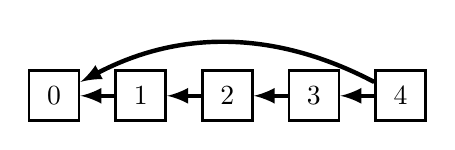
\begin{tikzpicture}[xscale=1.1]
      \foreach \i [count=\x] in {0, 1, 2, 3, 4} {%
        \node[smallsquare] (\i) at (\x, 0) {$\i$};
      }
      \draw[dep] (1) to (0);
      \draw[dep] (2) to (1);
      \draw[dep] (3) to (2);
      \draw[dep, bend right] (4) to (0);
      \draw[dep] (4) to (3);
    \end{tikzpicture}
    \caption{$G_1$}\figlabel{DeadlockBPaxosExampleG1}
  \end{subfigure}
  \hspace{1in}%
  \begin{subfigure}[b]{0.3\textwidth}
    \centering
    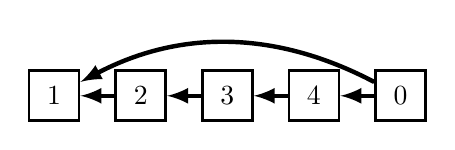
\begin{tikzpicture}[xscale=1.1]
      \foreach \i [count=\x] in {1, 2, 3, 4, 0} {%
        \node[smallsquare] (\i) at (\x, 0) {$\i$};
      }
      \draw[dep, bend right] (0) to (1);
      \draw[dep] (0) to (4);
      \draw[dep] (2) to (1);
      \draw[dep] (3) to (2);
      \draw[dep] (4) to (3);
    \end{tikzpicture}
    \caption{$G_2$}\figlabel{DeadlockBPaxosExampleG2}
  \end{subfigure}

  \vspace{0.2in}

  \begin{subfigure}[b]{0.3\textwidth}
    \centering
    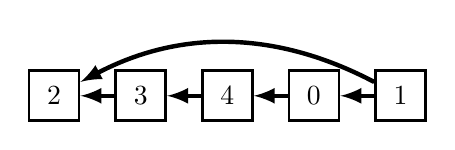
\begin{tikzpicture}[xscale=1.1]
      \foreach \i [count=\x] in {2, 3, 4, 0, 1} {%
        \node[smallsquare] (\i) at (\x, 0) {$\i$};
      }
      \draw[dep] (0) to (4);
      \draw[dep] (1) to (0);
      \draw[dep, bend right] (1) to (2);
      \draw[dep] (3) to (2);
      \draw[dep] (4) to (3);
    \end{tikzpicture}
    \caption{$G_3$}\figlabel{DeadlockBPaxosExampleG3}
  \end{subfigure}
  \hspace{1in}%
  \begin{subfigure}[b]{0.3\textwidth}
    \centering
    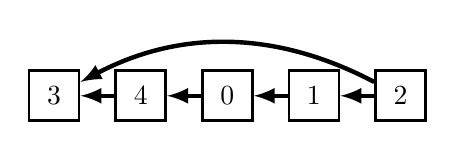
\begin{tikzpicture}[xscale=1.1]
      \foreach \i [count=\x] in {3, 4, 0, 1, 2} {%
        \node[smallsquare] (\i) at (\x, 0) {$\i$};
      }
      \draw[dep] (0) to (4);
      \draw[dep] (1) to (0);
      \draw[dep] (2) to (1);
      \draw[dep, bend right] (2) to (3);
      \draw[dep] (4) to (3);
    \end{tikzpicture}
    \caption{$G_4$}\figlabel{DeadlockBPaxosExampleG4}
  \end{subfigure}

  \vspace{0.2in}

  \begin{subfigure}[b]{0.3\textwidth}
    \centering
    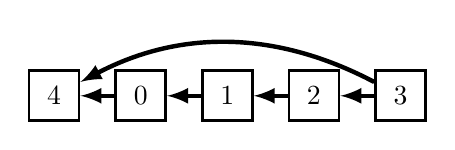
\begin{tikzpicture}[xscale=1.1]
      \foreach \i [count=\x] in {4, 0, 1, 2, 3} {%
        \node[smallsquare] (\i) at (\x, 0) {$\i$};
      }
      \draw[dep] (0) to (4);
      \draw[dep] (1) to (0);
      \draw[dep] (2) to (1);
      \draw[dep] (3) to (2);
      \draw[dep, bend right] (3) to (4);
    \end{tikzpicture}
    \caption{$G_5$}\figlabel{DeadlockBPaxosExampleG5}
  \end{subfigure}

  \caption{A Deadlock BPaxos deadlock}%
  \figlabel{DeadlockBPaxosExample}
\end{figure}
}

Imagine BPaxos node $S$ attempts to recover $I_0$. $\QuorumMajoritySize$
acceptors have voted for $\deps{0} = \set{4}$, but $o_2$ voted for $\set{1,
4}$. Thus, $S$ attempts to recover $I_1$. $\QuorumMajoritySize$ acceptors have
voted for $\deps{1} = \set{0}$, but $o_3$ voted for $\set{0, 2}$, so $S$
attempts to recover $I_2$. This continues until $S$ attempts to recover $I_4$.
$\QuorumMajoritySize$ acceptors have voted for $\deps{4} = \set{3}$, but $o_1$
voted for $\set{0, 3}$, so $S$ attempts to recover $I_0$. This is a deadlock.

Moreover, based on the order in which the $4$ failed nodes processed the five
commands, any four of the five commands could have been chosen. For example, if
the four failed nodes saw the commands in the order $0, 1, 2, 3, 4$, then the
commands $1, 2, 3, 4$ could have been committed on the fast path in round 0.
Or, if the four failed nodes saw the commands in the order $1, 2, 3, 4, 0$,
then the commands $2, 3, 4, 0$ could have been committed on the fast path in
round 0. Because these four nodes have failed, it is impossible for us to know
the order in which they processed the five commands, so it is impossible for us
to know which subset of the commands may have been committed. This shows that
there is no simple fix to \algoref{DeadlockBPaxos} that would allow a Deadlock
BPaxos node to resolve the deadlock.

\TODO[mwhittaker]{%
  There is still one small annoying detail not fully explained in this section.
  It might be possible that in the last else case of \algoref{DeadlockBPaxos},
  a node learns that $R.i$ has already been chosen, but it doesn't know what
  dependencies it has been chosen with. I think that this is actually
  impossible, but I'm not 100\% sure. To be super duper sure that it is
  impossible, we just have to make sure that whenever a node learns that an
  instance has been chosen, it also learns the value that was chosen. This is
  not at all hard to do, but it makes the protocol a little bit more
  cumbersome.
}


As with Fast \BPaxos{}, if $k = -1$ (\lineref{McbKEqualsNegativeOne}), if $k
> 1$ (\lineref{McbKGreaterThanZero}), or if $k = 0$ and there does not exist
$\maj{f+1}$ matching values (\lineref{McbNoMajority}), recovery is
straightforward.

Otherwise, there does exist a $v' = (x, \deps{v_x})$ voted for by at least
$\maj{f+1}$ acceptors in round $0$ (\lineref{McbMajority}). As with Fast
\BPaxos{}, $v'$ may have been chosen in round $0$, so the proposer \emph{must}
propose $v'$ in order to maintain the consensus invariant. But $\deps{v_x}$ may
not be the union of dependencies computed by $f+1$ dependency service nodes, so
the proposer is simultaneously forced \emph{not} to propose $v'$ in order to
maintain the dependency invariant. Unanimous \BPaxos{} avoided this tension by
increasing the size of fast Phase 2 quorums.  Majority Commit \BPaxos{} instead
resolves the tension by performing a more sophisticated recovery procedure.  In
particular, the proposer does a bit of detective work to conclude either that
$v'$ was definitely not chosen in round $0$ (in which case, the proposer can
propose a different value) or that $\deps{v_x}$ happens to be a pruned set of
dependencies (in which case, proposer is safe to propose $v'$).

On \lineref{McbSendToDependencyService} and
\lineref{McbReceiveFromDependencyService}, the proposer sends $x$ and $v_x$ to
the dependency service nodes co-located with the acceptors in $A$ (i.e.\ the
$f+1$ acceptors from which the proposer received \msgfont{Phase1b} messages).
Then proposer then computes the union of the returned dependencies, called
$\deps{v_x}_A$. Note that this communication can be piggybacked on the
\msgfont{Phase1a} messages that the proposer previously sent to avoid the extra
round trip of communication.
%
Also note that $\deps{v_x}$ was returned by $\maj{f+1}$ nodes in $A$, so
$\deps{v_x}$ is a subset of $\deps{v_x}_A$.

Next, the proposer enters a for loop in an attempt to prune $\deps{v_x}_A$
until it is equal to $\deps{v_x}$. That is, the proposer attempts to construct
a set of vertices $P$ such that $\deps{v_x} = \deps{v_x}_A - P$ is a set of
pruned dependencies. For every, $v_y \in \deps{v_x}_A - \deps{v_x}$, the
proposer first recovers $v_y$ if it does not know if a value has been chosen in
vertex $v_y$ (\lineref{McbRecoverVy}). After recovering $v_y$, assume the
proposer learns that $v_y$ is chosen with command $y$ and dependencies
$\deps{v_y}$. If $y = \noop$ or if $v_x \in \deps{v_y}$, then the proposer can
safely prune $v_y$ from $\deps{v_x}_A$, so it adds $v_y$ to $P$
(\lineref{McbPruneVy}).

Otherwise, the proposer contacts some quorum $A'$ of acceptors
(\lineref{McbContactAPrime}). If any acceptor $a_j$ in $A'$ knows that vertex
$v_x$ has already been chosen, then the proposer can abort the recovery of
$v_x$ and retrieve the chosen value directly from $a_j$
(\lineref{McbAbortRecovery}). Otherwise, the proposer concludes that no value
was chosen in $v_x$ in round $0$ and is free to propose any value that
maintains the pruned dependency invariant (\lineref{McbNothingChosen}). We will
explain momentarily why the proposer is able to make such a conclusion. It is
not obvious. Note that the proposer can piggyback its communication with $A'$
on its \msgfont{Phase1a} messages.

Finally, if the proposer exits the for loop, then it has successfully pruned
$\deps{v_x}_A$ into $\deps{v_x}_A - P = \deps{v_x}$ and can safely propose it
without violating the consensus or pruned dependency invariant
(\lineref{McbSuccessfulPruning}).  As described above, when the proposer sends
a \msgfont{Phase2a} message with value $v'$, it also includes the values chosen
in every instance in $P$.

We now return to \lineref{McbNothingChosen} and explain how the proposer is
able to conclude that $v'$ was not chosen in round $0$. On
\lineref{McbNothingChosen}, the proposer has already concluded that $v_y$ was
not chosen with $\noop$ and that $v_x \notin \deps{v_y}$. By the pruned
dependency invariant, $\deps{v_y} = \deps{v_y}_{D} - P'$ is a set of pruned
dependencies where $\deps{v_y}_{D}$ is a set of dependencies computed by a set
$D$ of $f+1$ dependency service nodes. Because $v_x \notin \deps{v_y}_{D} -
P'$, either $v_x \notin \deps{v_y}_{D}$ or $v_x \in P'$.

$v_x$ cannot be in $P'$ because if $v_y$ were chosen with dependencies
$\deps{v_y}_{D} - P'$, then some quorum of acceptors would have received $P'$
and learned that $v_x$ was chosen. But, when the proposer contacted the quorum
$A'$ of acceptors, none knew that $v_x$ was chosen, and any two quorums
intersect.

Thus, $v_x \notin \deps{v_y}_{D}$. Thus, every dependency service node in $D$
processed instance $v_y$ before instance $v_x$. If not, then a dependency
service node in $D$ would have computed $v_x$ as a dependency of $v_y$.
However, if every dependency service node in $D$ processed $v_y$ before $v_x$,
then there cannot exist a fast Phase 2 quorum of dependency service nodes that
processed $v_x$ before $v_y$. In this case, $v' = (x, \deps{v_x})$ could not
have been chosen in round $0$ because it necessitates a fast Phase 2 quorum of
dependency service nodes processing $v_x$ before $v_y$ because $v_y \notin
\deps{v_x}$.

\subsection{Ensuring Liveness}
Majority Commit \BPaxos{} is safe, but it is not very live. There are certain
failure-free situations in which Majority Commit \BPaxos{} can permanently
deadlock. The reason for this is \lineref{McbRecoverVy} in which a proposer
defers the recovery of one vertex for the recovery of another. There exist
executions of Majority Commit \BPaxos{} with a chain of vertices $v_1, \ldots,
v_m$ where the recovery of every vertex $b_i$ depends on the recovery of
vertex $v_{i+1 \bmod m}$.

We now modify Majority Commit \BPaxos{} to prevent deadlock.
%
First, we change the condition under which a value is considered chosen on the
fast path. A proposer considers a value $v = (x, \deps{v_x})$ chosen on the
fast path if a fast Phase 2 quorum $F$ of acceptors voted for $v$ in round $0$
\emph{and} for every vertex $v_y \in \deps{v_x}$, there exists a quorum  $A
\subseteq F$ of $f + 1$ acceptors that knew $v_y$ was chosen at the time of
voting for $v$.
%
Second, when an acceptor $a_i$ sends a \msgfont{Phase2b} vote in round $0$ for
value $v = (x, \deps{v_x})$, $a_i$ also includes the subset of vertices in
$\deps{v_x}$ that $a_i$ knows are chosen, as well as the values chosen in these
vertices.
%
Third, proposers execute \algoref{DeadlockBPaxos} but with
the lines of code shown in \algoref{MajorityCommitBPaxos} inserted after line
4.

\newcommand{\nullbot}{\textsf{null}}

\begin{algorithm*}[ht]
  \caption{%
    Majority Commit \BPaxos{} Proposer. Pseudocode for initiating recovery and
    handling \msgfont{Phase2B} messages is ommitted because it is identical to
    the pseudocode in \algoref{FastPaxosProposer}.
  }%
  \algolabel{MajorityCommitBPaxos}
  \begin{algorithmic}[1]
    \GlobalState a value $v$, initially \nullbot{}
    \GlobalState a round $i$, initially $-1$

    \Upon{receiving \msg{Phase1B}{i, vr, vv} from $f+1$ acceptors $A$}
      \State $k \gets$ the largest $vr$ in any \msg{Phase1B}{i, vr, vv}
      \If{$k = -1$} \linelabel{McbKEqualsNegativeOne}
        \State $v \gets$ an arbitrary value satisfying the dependency invariant
        % Addresses Reviewer 3.
        %
        % > I am unsure why at line 21 of Algorithm 1, the propose is sending to at
        % > least $f+1$ acceptors instead of all acceptors. As $f$ of the acceptors
        % > may crash, so sending to all acceptors in important.
        \State send \msg{Phase2A}{i, v} to \markrevisions{the acceptors}
      \ElsIf{$k > 0$} \linelabel{McbKGreaterThanZero}
        \State $v \gets$ the corresponding $vv$ in round $k$
        % Addresses Reviewer 3.
        %
        % > I am unsure why at line 21 of Algorithm 1, the propose is sending to at
        % > least $f+1$ acceptors instead of all acceptors. As $f$ of the acceptors
        % > may crash, so sending to all acceptors in important.
        \State send \msg{Phase2A}{i, v} to \markrevisions{the acceptors}
      \ElsIf{%
        there are $\maj{f + 1}$ \msg{Phase1B}{i, 0, v'} messages for some value
        $v'$
      } \linelabel{McbMajority}
        \State $(x, \deps{v_x}) \gets v'$
               \linelabel{McbUnwrapVPrime}

        \State send $v_x$ and $x$ to the dependency service nodes co-located
               with the acceptors in $A$
               \linelabel{McbSendToDependencyService}
        \State $\deps{v_x}_A \gets$ the union of the dependencies returned by
               these dependency service nodes
               \linelabel{McbReceiveFromDependencyService}
        \State
        \State $P \gets \emptyset$
        \For{$v_y \in \deps{v_x}_A - \deps{v_x}$}
          \If{we don't know if $v_y$ is chosen}
            \State recover $v_y$, blocking until $v_y$ is recovered
                   \linelabel{McbRecoverVy}
          \EndIf
          \If{$v_y$ chosen with $\noop$ or with $v_x \in \deps{v_y}$}
            \State $P \gets P \cup \set{v_y}$
                   \linelabel{McbPruneVy}
          \Else{}
            \State contact a quorum $A'$ of acceptors
                   \linelabel{McbContactAPrime}
            \If{an acceptor in $A'$ knows $v_x$ is chosen}
              \State abort recovery; $v_x$ has already been chosen
                     \linelabel{McbAbortRecovery}
            \Else{}
              \State $v \gets$ an arbitrary value satisfying the dependency invariant
                     \linelabel{McbNothingChosen}
              % Addresses Reviewer 3.
              %
              % > I am unsure why at line 21 of Algorithm 1, the propose is sending to at
              % > least $f+1$ acceptors instead of all acceptors. As $f$ of the acceptors
              % > may crash, so sending to all acceptors in important.
              \State send \msg{Phase2A}{i, v} to \markrevisions{the acceptors}
            \EndIf{}
          \EndIf{}
        \EndFor{}
        \State $v \gets v'$
        \State send \msg{Phase2A}{i, v} and the values chosen in $P$ to at
               least $f + 1$ acceptors
               \linelabel{McbSuccessfulPruning}
      \Else{} \linelabel{McbNoMajority}
        \State $v \gets$ an arbitrary value satisfying the dependency invariant
        % Addresses Reviewer 3.
        %
        % > I am unsure why at line 21 of Algorithm 1, the propose is sending to at
        % > least $f+1$ acceptors instead of all acceptors. As $f$ of the acceptors
        % > may crash, so sending to all acceptors in important.
        \State send \msg{Phase2A}{i, v} to \markrevisions{the acceptors}
      \EndIf
    \EndUpon
  \end{algorithmic}
\end{algorithm*}


We now explain \algoref{MajorityCommitBPaxosProposerModification}. On
\lineref{McbmM}, the proposer computes the subset $M \subseteq A$ of acceptors
that voted for $v'$ in round $0$. On \lineref{McbmObliviousM}, the proposer
determines whether there exists some instance $v_y \in \deps{v_x}$ such that no
acceptor in $M$ knows that $v_y$ is chosen. If such an $v_y$ exists, then $v'$
was not chosen in round $0$. To see why, assume for contradiction that $v'$ was
chosen in round $0$. Then, there exists some fast Phase 2 quorum $F$ of
acceptors that voted for $v'$ in round $0$, and there exists some quorum $A'
\subseteq F$ of acceptors that know $v_y$ has been chosen. However, $A$ and
$A'$ intersect, but no acceptor in $A$ both voted for $v'$ in round $0$ and
knows that $v_y$ was chosen.  This is a contradiction. Thus, the proposer is
free to propose any value satisfying the dependency invariant.

Next, it's possible that the proposer was previously recovering instance $v_z$
with value $(z, \deps{v_z})$ and executed \lineref{McbRecoverVy} of
\algoref{MajorityCommitBPaxos}, deferring the recovery of instance $v_z$ until
after the recovery of instance $v_x$.
%
If so and if $v_z \in \deps{v_x}$, then some acceptor $a_j \in M$ knows that
$v_z$ is chosen. Thus, the proposer can abort the recovery of instance $v_z$
and retrieve the chosen value directly from $a_j$ (\lineref{McbmVzinVx}).
%
Otherwise, $v_z \notin \deps{v_x}$. In this case, no value was chosen in round
$0$ of instance $v_z$, so the proposer is free to propose any value satisfying
the pruned dependency invariant in instance $v_z$. Here's why. $v_z \notin
\deps{v_x}$, so every dependency service node co-located with an acceptor in
$M$ processed $v_x$ before $v_z$. $|M| \geq \maj{f+1}$, so there strictly fewer
than $f + \maj{f+1}$ remaining dependency service nodes that could have
processed $v_z$ before $v_x$.  If the proposer was recovering instance $v_z$
but deferred to the recovery of instance $v_x$, then $v_x \notin \deps{v_z}$.
In order for $v_z$ to have been chosen in round $0$ with $v_x \notin
\deps{v_y}$, it requires that at least $f + \maj{f}$ dependency service nodes
processed $v_z$ before $v_x$, which we just concluded is impossible. Thus,
$v_z$ was not chosen in round $0$.

Majority Commit \BPaxos{} is deadlock free for the following reason. If a
proposer is recovering instance $v_z$ and defers to the recovery of instance
$v_x$, then either the proposer will recover $v_x$ using
\lineref{McbmObliviousM} of \algoref{MajorityCommitBPaxosProposerModification}
or the proposer will recover $v_z$ using \lineref{McbmVzInVx} or
\lineref{McbmVzNotInVx} of \algoref{MajorityCommitBPaxosProposerModification}.
In either case, any potential deadlock is avoided.

\subsection{EPaxos and Caesar}
EPaxos~\cite{moraru2013there} and Caesar~\cite{arun2017speeding} are two
generalized multi-leader protocols that implement tension resolution. EPaxos is
very similar Majority Commit \BPaxos{} with the Basic EPaxos optimization from
\secref{BasicEPaxosOptimization} used to reduce fast Phase 2 quorum sizes by 1.
Majority Commit \BPaxos{} and EPaxos both prune dependencies and perform a
recursive recovery procedure with extra machinery to avoid deadlocks.
%
Caesar improves on EPaxos in two dimensions. First, much like Atlas, a Caesar
proposer does not require that a fast Phase 2 quorum of acceptors vote for the
exact same value in order to take the fast path. Second, Caesar avoids a
recursive recovery procedure. Caesar accomplishes this using a combination of
logical timestamps and carefully placed barriers in the protocol.
